\section{Extreme significant wave heights}
The maximum measured and modeled wave heights are associated with storms. However, because it takes both a high wind speed 
and a large fetch and duration to produce large waves, the largest waves are generally caused by storms with high winds that move 
at a speed close to the group speed of the dominant waves. Figure \ref{fig:10yearHsWW3} illustrates that $H_s$ generally exceeds 16~m once 
every 10 years in a good fraction of the North Atlantic: the biggest waves on Earth are found between Ireland and Iceland. 

%%%%%%%%%%%%% figure
\begin{figure}[htb]
\centerline{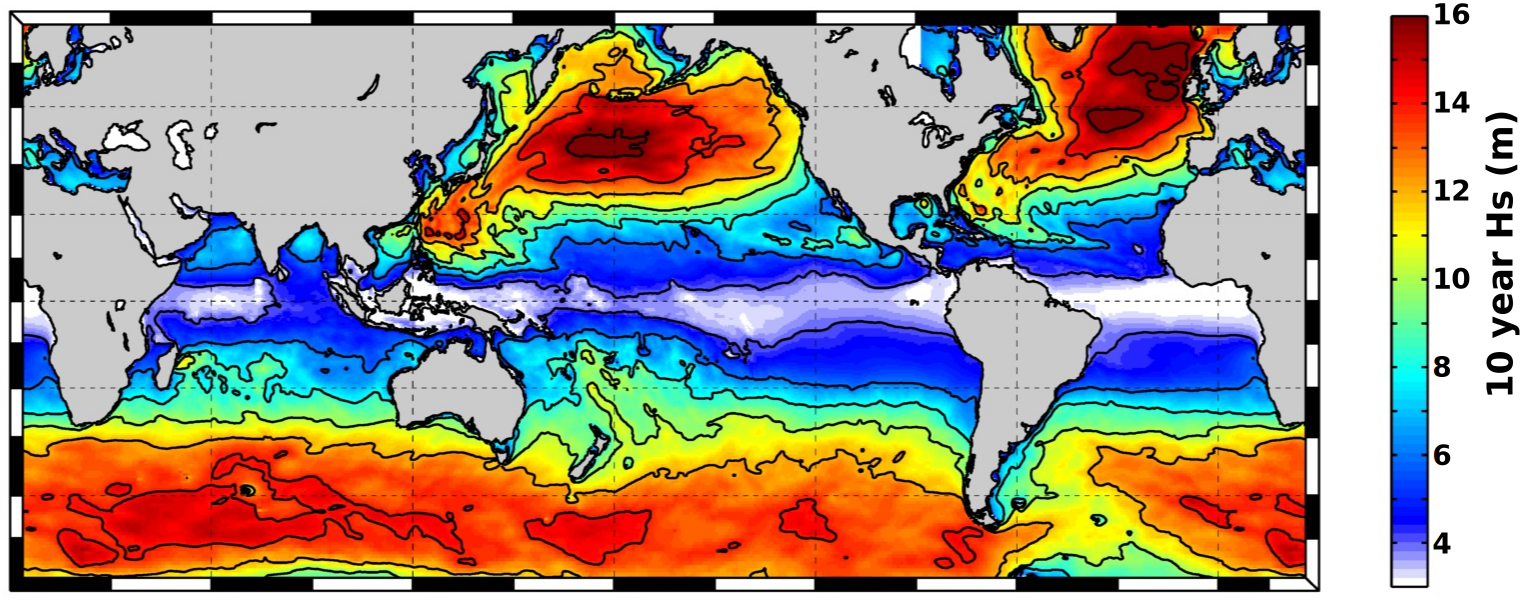
\includegraphics[width=1.0\textwidth]{FIGURES/10yearHs_WW3.pdf}}
  \caption{Estimate of the 10-year significant wave height (the expected maximum value of $H_s$ that occurs every 10 years) based on a 
  30-year hindcast, from 1985 to 2015, using WAVEWATCH III forced by CFSR winds \cite{Saha&al.2010}, and fitting yearly maxima with a Generalized Extreme Value distribution. Image courtesy of J. Stopa.}
  \label{fig:10yearHsWW3}
\end{figure}
%%%%%%%%%%%%% end of figure
Wind speeds in tropical storms can be much faster, probably exceeding 70 m/s in the Typhoon Haiyan that hit the Philippines in 2014, but
the motion of these storms does not generally lead to the largest wave heights \citep[see also][]{Quilfen&al.2010}. 

The pattern on maxima is thus very different in the tropics where they are related to individual storm tracks, and in the 
higher latitudes where the broad structures of extra-tropical storm give large values of $H_s$ over a wide region. 
For example the maximum in the Gulf of Mexico (around 11~m) in figure \ref{fig:10yearHsWW3} is the result of the passage of a 
single storm: Hurricane Katrina, which led to widespread damage and coastal flooding \citep[e.g.][]{Resio&Westerink2008}. 
Using a different time frame, say around 1900 instead of 2000, would probably have highlighted a different maximum, around Galveston, Texas, 
associated to the 1900 hurricane that hit that part of the coast. 
Because it is not possible to know where the next tropical storm tracks will be, an assessment of coastal hazards usually uses 
empirical storm tracks with randomly shifted positions to investigate the local impact of a track displacement. 

%%%%%%%%%%%%% figure
\begin{figure}[htb]
\centerline{\includegraphics[width=1.0\textwidth]{FIGURES/Quirin_winds.pdf}}
  \caption{Modeled winds (top panel, every 12 hours from 13 February at 00h00 to  14 February at  12h00) and  observed  (bottom) 
  during the development of the storm Quirin in February 2011. The light blue and magenta contours  give the 
  limit of tropical storm  ($U_{10}>$  24.5 m/s) and hurricane force ($U_{10}>$  32.7 m/s) wind speeds.}
  \label{fig:Quirin_winds}
\end{figure}
%%%%%%%%%%%%% end of figure
The highest-ever measured value of $H_s$ is  20.1~m, using 1-Hz altimeter data from Jason 2. This measurement was made over the North-Atlantic storm 
Quirin, in February 2011. Although the wind speed probably approached 40~m/s, these waves were associated to a storm travelling at the right 
speed across the Atlantic, amplifying the dominant waves along its path, which resulted in an effective fetch exceeding 2000~km and a duration 
larger than 48 hours. 


%%%%%%%%%%%%% figure
\begin{figure}[htb]
\centerline{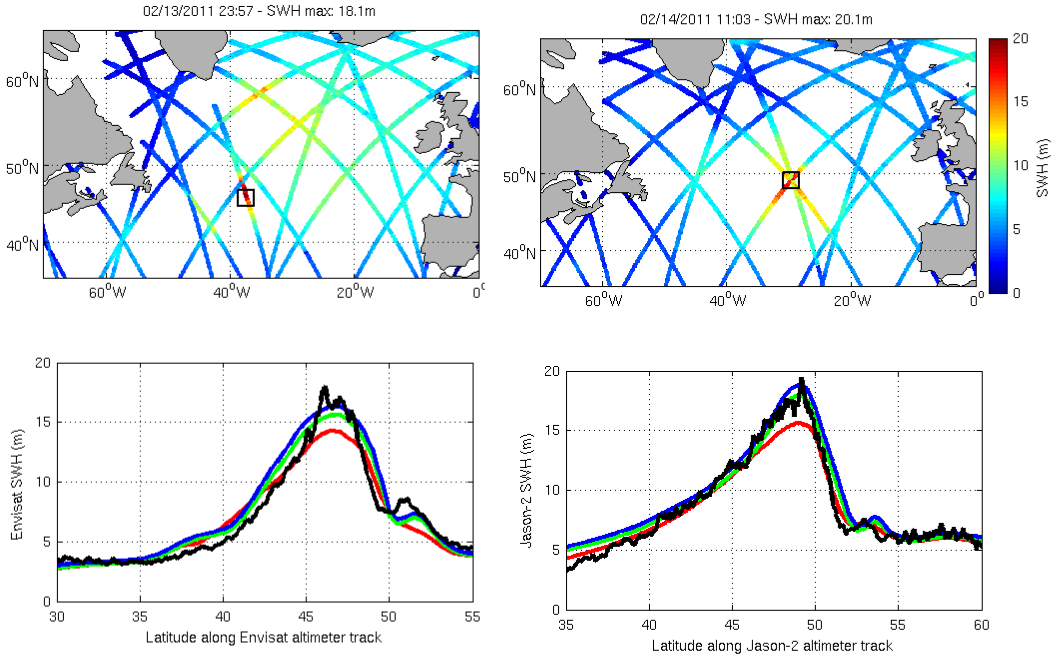
\includegraphics[width=0.8\textwidth]{FIGURES/Quirin_waves.pdf}}
  \caption{Measured $H_s$ from altimeters on 13 and 14 February 2012. Bottom: measured (black) and modeled  (color) wave heights using 
  different wind forcings: red is ECMWF operational analyses, green is NOAA/NCEP analyses, and blue is the wind speed from NOAA/NCEP enhanced by 10\%.}
  \label{fig:Quirin_waves}
\end{figure}
%%%%%%%%%%%%% end of figure

For different regions of the world, different storms have been recorded as particularly severe. In the United States, these are usually associated to hurricanes 
such as the 1969 Hurrican Camille, or combination of North-Easter storms and hurricanes \cite[e.g. the 1991 Perfect Storm that inspired the movie, see][]{Bromirski2001}. 

\section{Physical processes at high wind speeds}
Parameterizations in wave models have been developed for wind speeds ranging from 5 m/s \citep{Snyder&al.1981} to 20 m/s or so. At higher wind speeds, 
the physical properties of the sea surface and the airflow above it is expected to be significantly different. The sea surface is 
characterized by the presence of foam and spray \citep[e.g.][]{Holthuijsen&al.2012}. In particular, Kelvin-Helmholz or other 
instabilities can play a leading role \cite{Soloviev&al.2014}. It may be surprising that wave models actually work pretty well for $H_s$ up to 18~m \citep{Rascle&Ardhuin2013},
but this is probably because these large waves mostly occur in regions when the wind is not so extreme, but rather where storms move with the waves. 

\section{Variability and trends of sea state parameters}
As waves are related to ocean winds, so does the variability in wind speeds strongly impacts the waves. The El-Nino Southern Oscillation has a very big 
impact on waves across the Pacific \citep{Bromirski&al.2005,Stopa&Cheung2014}, and North Atlantic storms are strongly affected by the North Atlantic 
Oscillations \citep[e.g.][]{Dodet&al.2010,Charles&al.2012}. Given this very large interannual variability, it is very difficult to estimate 
long term trends, such as associated to global change. The studies by \cite{Hemer&al.2013}, \cite{Wang&al.2014}, and \cite{Shimural&al.2016b} show that 
the shift of high winds speed regimes towards high latitude generally leads to a reduction in wave height at latitudes under 50 degrees, and an increase 
at higher latitudes. However, the trends for extremes are a complex combination of the number and intensity of tropical storms with the extra tropical 
storms, so that the extreme wave heights may rise in some regions and decrease in others \citep{Shimural&al.2016b}. The case of the Arctic is particular, 
with a general increase in wave height that is associated to a reduced extent of sea ice \citep{Stopa&al.2016b}.
